\chapter{Brief overview of the next study}

Based on the feedback we got from the initial study, we have developed a second glove prototype employing solutions suggested in the results of previous usability testing. 

\section{Data Glove Prototype II}

The second iteration of the glove has improved in hardware, software performance, design and cost\footnote{As seen in Figure \ref{fig:prototype2}}.

\begin{figure}
    \begin{subfigure}
        \centering
        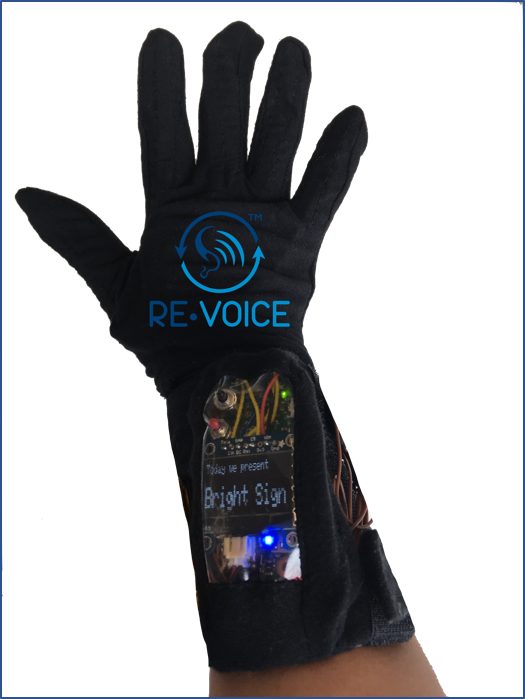
\includegraphics[width=0.5\textwidth]{./assets/img/Glove}
        \caption{Eat}
        \label{fig:glove}
    \end{subfigure}
    \begin{subfigure}
        \centering
        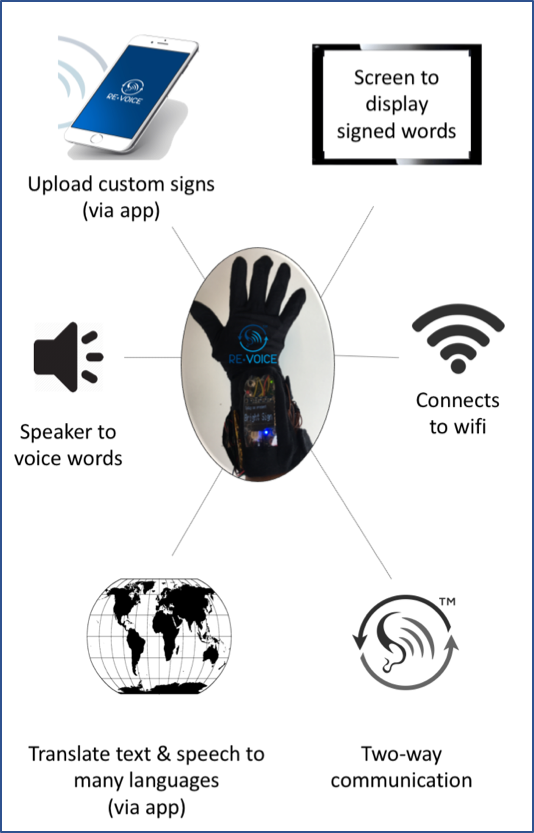
\includegraphics[width=0.5\textwidth]{./assets/img/GloveFeatures}
        \caption{Hungry}
        \label{fig:glovefeatures}
    \end{subfigure}
    \caption{Examples of a test subject making hand gestures while wearing the Data Glove}
    \label{fig:prototype2}
\end{figure}

\begin{itemize}
\item \textbf{Hardware:} Raspberry Pi Zero with an embedded circuit, speaker, OLED screen and power supply all on one board.

\item \textbf{Software:} Machine learning employed to allow each user to train the glover to their own version of sign language and to their personal motor ability. Speech output can be set in any language. 

\item \textbf{Design:} All hardware embedded in special channels sewed in the lining of the glove.  Circuit is insulated with non-conductive and fire resistant fabric.  Circuit is removable to enable washing of the glove. Glove fabric is stretchable and soft.  

\item \textbf{Cost:} Hardware cost was reduced by half. Design cost increased because the glove was custom made. Software had to be paired with cloud computing web application which requires an ongoing subscription. 
\end{itemize}

Testing was done with two different groups of users and in two locations:

\section{No Barriers Summit: Innovation Village, Lake Tahoe, June 2017}

No Barriers Summit is an annual event bringing together assistive technology and individuals with different disabilities to interact with the technology in an open four- day exhibition. I was invited to give a talk about my data glove and showcase it in the exhibition. The data glove was used by a number of adults with speech disabilities, hearing and visual impairment\footnote{As in Figure \ref{fig:participants}}.

\begin{figure}
    \begin{subfigure}
        \centering
        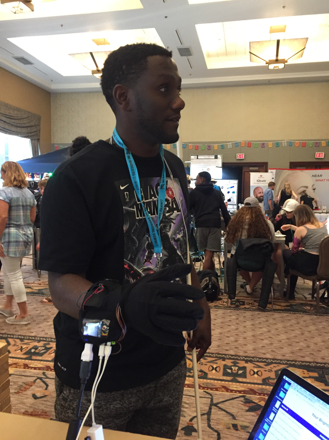
\includegraphics[width=0.5\textwidth]{./assets/img/ParticipantA}
        \caption{Eat}
        \label{fig:participanta}
    \end{subfigure}
    \begin{subfigure}
        \centering
        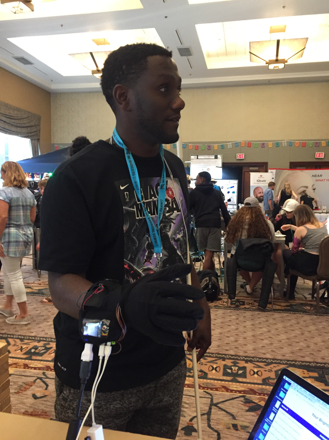
\includegraphics[width=0.5\textwidth]{./assets/img/ParticipantA}
        \caption{Hungry}
        \label{fig:participantb}
    \end{subfigure}
    \caption{Examples of a test subject making hand gestures while wearing the Data Glove}
    \label{fig:participants}
\end{figure}

The task was to demonstrate, to one participant at a time, how to record custom sign language hand gestures. The participant then puts on the glove, presses the record button, makes a dynamic hand gesture, then saves the gesture under a name of their choice. Next, the participant chooses a language from a drop-down menu for the output speech. Finally, the participant makes the same dynamic hand gesture he has recorded and a word is displayed on the screen and spoken out through the speaker in the language selected. 

We had seven participants who were patient enough to go through the 20 minute process. Accuracy rate was 100\% with no errors. This is because the glove is being trained and tested by the same person, so the errors that occur because of hand gesture variations were eliminated in this incident.  

Participant reactions varied between amazement, and feeling enabled.  They had a sense of achievement when they trained the glove and the output was accurate. 

Observation revealed that the participant with visual impairment did not know which buttons to press, buttons were colour coded. Connectivity to the web application (where the machine learning happened) was very difficult using a public network so we had to keep the glove connected to the computer via a wire, although it was designed to operate as a stand-alone device. Also, there was no feedback on the glove that informed the participant of which mode the glove was on, training, classifying or processing.

Direct feedback from several participants suggested that they prefer keeping eye contact while signing and don’t have a use for the screen. Although the screen is not essential for communication, we feel that it confirms to the hearing-impaired signer that what he is signing is indeed what is being spoken out through the speaker. This feature was especially useful when I used the glove to sign to a Korean crowd and set the speech out to Korean and didn’t understand the speech. 

\section{Charlton Park Academy: Communication Works, London, July 2017}

Charlton Park Academy is an inclusive school for children with different needs. Most of the students in the school need assistive technology to communicate. I was invited to give a talk about my data glove and to showcase my data glove in an exhibition for assistive technology called ``Communication Works'' amongst a wide range of assistive technology designed to enable communication. Tablets with special communication apps were on show and cost a minimum of £2K to £9K with a monthly subscription.  The impact of the talk was positive and I had queue of parents requesting to include their children in the glove studied. Parents expressed that they are interested in acquiring the data glove for their children. 

When asked about what their children currently use and what were the drawbacks, most parents had similar responses.  All children with non-verbal disabilities in the school used special tablets with communication apps. Parents' main concerns were: having to limit the use of tablets with their children, resorting to lock the tablet to restrict its use to the communication app which causes frustration to the children.  Another disadvantage was that children don’t learn how to sign or have eye contact while interacting with the public. They hide behind the screen and often keep their eyes low or fixated on the screen. 

\section{Discussion:}

Collating feedback from both events, an outline for the next prototype has emerged.  Main issues to be addressed:

To add feedback on the glove to inform users of the three different software states: Record, Train, Save.  Feedback will be in the form of text appearing on the screen attached to the glove. 

To solve connectivity problems by adding a mobile module with a chip or a Bluetooth\texttrademark Low Energy (BLE) to replace WiFi\texttrademark. 

Change buttons to be different shapes rather than different colours to cater to the needs of visual impaired individuals.

Design a custom PCB with arm processor, built in text to speech synthesiser, speaker and screen. Consider circuits used for wearable technology; such as flexible circuits, printed circuits and embedded censors. 

Power supply with narrow band technology to reduce power consumption especially if a GSM/SIM chip is added to the circuit.  Mobile modules require power to connect and consume energy to maintain connectivity.  








